% Section 3 - Services
% Roberto Masocco <roberto.masocco@uniroma2.it>
% May 2, 2026

% ### Services ###
\section{Services}
\graphicspath{{figs/section3/}}

% --- ROS 2 services ---
\begin{frame}{ROS 2 services}{Basic client-server paradigm}
  \justifying
  ROS 2 builds on the basic one-way messages adding two more communication paradigms: the first is the \textbg{service}. It allows nodes to establish quick and simple \textbg{client-server} communications.
  \begin{figure}
    \centering
    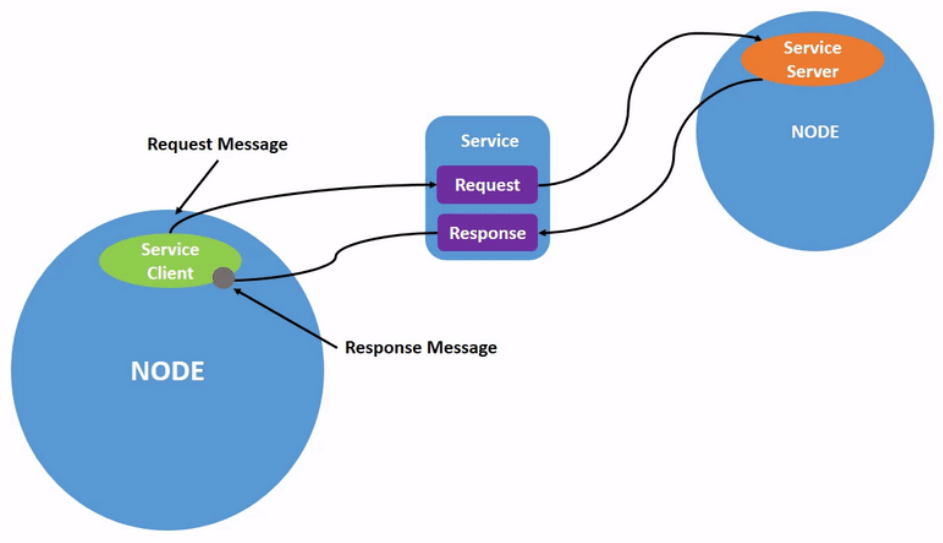
\includegraphics[scale=.33]{ros2Srv.png}
    \caption{Two nodes acting as service \emph{client} and \emph{server}.}
    \label{fig:ros2srv}
  \end{figure}
\end{frame}
\begin{frame}{ROS 2 services}{Communication overview}
  \justifying
  \begin{enumerate}
    \item The \textbg{client} sends a \textbg{request message} to the server.
    \item The \textbg{server} receives the request and processes it.
    \item Meanwhile, the \textbg{client} may either \textbg{block} waiting for the response or \textbg{synchronously poll} it.
    \item When done, the \textbg{server} sends a \textbg{response message} to the client.
    \item If waiting, the \textbg{client} awakes when it receives the response.
  \end{enumerate}
\end{frame}
\begin{frame}{ROS 2 services}{CLI introspection tools}
  \justifying
  The main command is \texttt{ros2 service} with the following verbs.
  \begin{itemize}
    \item \texttt{list} Lists all active services.
    \item \texttt{type} Prints the service type.
    \item \texttt{find} Lists active services of the given type.
    \item \texttt{call} Calls the service with the request defined in the command line.
  \end{itemize}
\end{frame}
\begin{frame}{ROS 2 services}{Coding hints for servers and clients}
  \begin{block}{Servers}
    \justifying
    Similarly to topic subscriptions, requests are processed in appropriate \textbf{callbacks}, taking \textbf{two arguments}: the \textbf{request} containing input data and the \textbf{response} to be filled with output data. The \texttt{Service} object is only needed to handle the life cycle of the service.
  \end{block}
  \begin{block}{Clients}
    \justifying
    As per the previous dynamics, one has to \textbf{code each step} of the client side into their application using appropriate \textbf{ROS 2 APIs}. \textbf{The client object is used to send requests}, while \textbf{responses are handled as \texttt{std::future<T>} objects\footnote{\href{https://en.cppreference.com/w/cpp/thread/future}{\color{blue}\underline{\texttt{std::future<T>} - C++ Reference}}}}.
  \end{block}
\end{frame}
\begin{frame}{ROS 2 services}{Coding hints for futures}
  \justifying
  When handling \textbg{future objects}, \emph{e.g.}, when coding a \textbg{service client} waiting for a \textbg{response}, you may do one of the following:
  \begin{itemize}
    \item \textbg{go on with your code and check} if the future holds a value;
      \begin{itemize}
        \item \texttt{future.valid()} method;
      \end{itemize}
    \item \textbg{block waiting} for the future to get a value;
      \begin{itemize}
        \item \texttt{future.get()} method;
      \end{itemize}
    \item \textbg{wait for some time} for the future to get a value;
      \begin{itemize}
        \item \texttt{future.wait\_for()} method (recall the one for condition variables);
        \item \texttt{rclcpp::spin\_until\_future\_complete(node, future)} method.
      \end{itemize}
  \end{itemize}
\end{frame}
\begin{frame}{ROS 2 services}{Coding hints for futures}
  \justifying
  \begin{itemize}
    \item \texttt{spin\_until\_future\_complete(node, future)} (a method of the \texttt{Executor} classes) \textbg{spins an executor with the node until the future gets a value}.
      \begin{itemize}
        \item \textbg{Other ROS events keep being processed while waiting for the response to arrive.}
        \item \textbg{Use this only if no other thread is spinning an executor with the node.}
      \end{itemize}
    \item \texttt{future.wait\_for()} \textbg{blocks the calling thread} until either the future gets a \textbg{value} or the \textbg{timeout} occurs.
      \begin{itemize}
        \item \textbg{Use this only when another thread is spinning an executor with the node.}
      \end{itemize}
  \end{itemize}
\end{frame}
\begin{frame}{ROS 2 services}{Coding hints for futures}
  \begin{alertblock}{Deadlocks!}
    \justifying
    \textbr{A service response is a ROS event that must be handled, \emph{i.e.}, an executor must be spinning to get it.}\\
    \medskip
    \textbr{No executor running or the one available being blocked} (\emph{e.g.}, if waiting, blocking or not, for a service response inside a callback executed by a \texttt{SingleThreadedExecutor}) results in a \textbr{deadlock}.\\
    \medskip
    When waiting for futures, pay attention to either
    \begin{itemize}
      \item do so from \textbr{dedicated threads and not callbacks}, or
      \item use a properly configured \texttt{MultiThreadedExecutor}.
    \end{itemize}
  \end{alertblock}
\end{frame}

% --- Interface files - Services ---
\begin{frame}[fragile]{Interface files}{Services}
  \justifying
  The entire system is built on messages, so \textbg{combine two of them} in a single interface file, separated by \texttt{-{}-{}-}.\\
  Service file names end with \texttt{.srv}.
  \begin{columns}
    \column{.9\textwidth}
  % Listing: example_interfaces/srv/AddTwoInts service definition
    \begin{lstlisting}[language=ros2msg, caption=Definition of the \texttt{example\_interfaces/srv/AddTwoInts} service.]
# REQUEST
int64 a
int64 b
---
# RESPONSE
int64 sum
    \end{lstlisting}
  \end{columns}
\end{frame}

% --- Example - Simple service ---
\begin{frame}{Example}{Simple service}
  \begin{block}{}
    \centering
    Now go have a look at the \href{https://github.com/IntelligentSystemsLabUTV/ros2-examples/tree/jazzy/src/cpp/simple_service_cpp}{\color{blue}\underline{\texttt{ros2-examples/src/cpp/simple\_service\_cpp}}} package!
  \end{block}
\end{frame}
